%! Author = Ivan Chizhov
%! Date = 08.11.2022

% Preamble
\documentclass[colorthm]{../civarticle}
\usepackage[math]{blindtext}

\title{
    Блоковые шифры. Шифр ГОСТ 34.12-2018 "Кузнечик"\\
    %\small{(оформление окружений цветом и пр.)}%
}
\author{А.~С.~Сахаутдинова}
\if 0
\abstract{%
    \Blindtext[2][1]
}
\keywords{%
    \Blindtext[1][1]
}
\fi
% Document
\begin{document}
\blindmathtrue
\section{Введение}
\label{sec:thm-pif}

В современном мире цифровых технологий и глобальной информационной безопасности криптография играет ключевую роль в защите конфиденциальных данных. Особое место в этой области занимают блоковые шифры, представляющие собой метод преобразования блоков данных с использованием специально разработанных алгоритмов и ключей. Это эссе посвящено изучению и анализу наиболее значимых и влиятельных блоковых шифров, которые определили развитие современной криптографии.

Среди рассматриваемых шифров – классический DES и его усовершенствованная версия 3DES, широко используемые в финансовых и правительственных системах. Алгоритм AES, признанный мировым стандартом, заслуживает особого внимания благодаря своей надежности и эффективности. Российские стандарты ГОСТ 34.12-2018, представленные шифрами "Магма" и "Кузнечик", показывают уникальные подходы к обеспечению информационной безопасности. Шифры IDEA и IDEANXT, хотя и менее известны, представляют значительный интерес с точки зрения их структуры и принципов работы. А также шифр RC6, являющийся одним из финалистов конкурса AES, демонстрирует интересные инновационные решения в области криптографии.

Особое внимание в этом эссе уделено шифру "Кузнечик"\. Он представляет собой один из самых перспективных современных алгоритмов, объединяющий в себе сложность и высокий уровень безопасности. Анализ атак на "Кузнечик"\ не только позволяет оценить его устойчивость к криптоанализу, но и способствует пониманию общих принципов и вызовов, стоящих перед криптографической общественностью в области разработки и анализа блоковых шифров.


\section{Термины и определения}
Следующие определения и термины взяты из стандарта ГОСТ 34.12-2018 ~\cite{gost2018}.

\textbf{Алгоритм зашифрования}: Алгоритм, реализующий зашифрование, т. е. преобразующий открытый текст в шифртекст

\textbf{Алгоритм расшифрования}: Алгоритм, реализующий расшифрование, т. е. преобразующий шифртекст в открытый текст.

\textbf{Базовый блочный(блоковый) шифр}: Блочный шифр, реализующий при каждом фиксированном значении ключа одно обратимое отображение множества блоков открытого текста фиксированной длины в блоки шифртекста такой же длины.

\textbf{Блок}: Строка бит определенной длины.

\textbf{Блочный(блоковый) шифр}: Шифр из класса симметричных криптографических методов, в котором алгоритм зашифрования применяется к блокам открытого текста для получения блоков шифртекста.

\textbf{Зашифрование}: Обратимое преобразование данных с помощью шифра, которое формирует шифртекст из открытого текста.

\textbf{Итерационный ключ}: Последовательность символов, вычисляемая в процессе развертывания ключа шифра и определяющая преобразование на одной итерации блочного(блокового) шифра.

\textbf{Ключ}: Изменяемый параметр в виде последовательности символов, определяющий криптографическое преобразование.

\textbf{Открытый текст}: Незашифрованная информация.

\textbf{Развертывание ключа}: Вычисление итерационных ключей из ключа шифра.

\textbf{Расшифрование}: Операция, обратная к зашифрованию.

\textbf{Симметричный криптографический метод}: Криптографический метод, использующий один и тот же ключ для преобразования, осуществляемого отправителем. и преобразования, осуществляемого получателем.

\textbf{Шифр}: Криптографический метод, используемый для обеспечения конфиденциальности данных, включающий алгоритм зашифрования и алгоритм расшифрования.

\textbf{Шифртекст}: Данные, полученные в результате зашифрования открытого текста в целях скрытия его содержания.



\section{Описание шифров}

\begin{enumerate}
\item \textbf{DES и 3DES}

\textit{DES (Data Encryption Standard)}: Это блоковый шифр с размером блока 64 бита и длиной ключа 56 бит, разработанный в начале 1970-х годов. DES использует сеть Фейстеля, включающую 16 раундов шифрования. Несмотря на то что он считается устаревшим и уязвимым для атаки полным перебором ключей, DES оказал значительное влияние на развитие криптографии.

\textit{3DES (Triple DES)}: Это усовершенствование DES, предложенное для увеличения уровня безопасности. 3DES применяет алгоритм DES три раза к каждому блоку данных, используя два или три разных ключа, что обеспечивает общую длину ключа 112 или 168 бит.

\item \textbf{AES (Advanced Encryption Standard)}

\textit{AES}: Этот шифр был принят в качестве стандарта шифрования правительством США в 2001 году. AES является блоковым шифром с размером блока 128 бит и поддерживает ключи длиной 128, 192 или 256 бит. Алгоритм использует структуру, известную как сеть замены-перестановки, и включает несколько раундов шифрования (10, 12 или 14 в зависимости от длины ключа).

\item \textbf{ГОСТ 34.12-2018 "Магма"}

\textit{Магма}: Это российский стандарт блокового шифрования, принятый в 2018 году. Шифр работает с блоками по 64 бита и использует 256-битный ключ. Он основан на модифицированной сети Фейстеля и включает 32 раунда шифрования. 

\item \textbf{ГОСТ 34.12-2018 "Кузнечик"}

\textit{Кузнечик}: Также введен в 2018 году, "Кузнечик" является российским блоковым шифром с размером блока 128 бит и 256-битным ключом. Шифр использует сеть подстановок и перестановок, состоящую из 10 раундов. Он отличается от "Магмы" более сложной структурой и предназначен для использования в системах с высокими требованиями к безопасности.

\item \textbf{IDEA и IDEA NXT}

\textit{IDEA (International Data Encryption Algorithm)}: Это блоковый шифр, который был разработан в 1991 году. IDEA работает с блоками по 64 бита и использует 128-битный ключ. Шифр комбинирует операции из разных групп (сложение по модулю $2^{16}$, сложение по модулю $2^{32}$ и XOR) в 8 раундах.

\textit{IDEA NXT (ранее известный как FOX)}: Это улучшенная версия IDEA с увеличенным размером блока и длиной ключа, а также более сложной структурой.

\item \textbf{RC6}

\textit{RC6}: Разработанный RSA Security в 1998 году, RC6 является блоковым шифром, предложенным как кандидат на стандарт AES, но не выбранным в итоге. Он работает с блоками размером 128 бит и поддерживает ключи разной длины (128, 192 или 256 бит). RC6 похож на своего предшественника RC5 и использует комбинацию линейных и нелинейных операций в своих раундах. Основные элементы алгоритма включают в себя циклические сдвиги, сложение и умножение. 

\end{enumerate}



\section{Шифр "Кузнечик"\ }


Шифр "Кузнечик"\ (ГОСТ 34.12-2018), введен в действие в 2018 году, заменив предыдущий стандарт ГОСТ Р 28147-89. Этот современный российский блоковый шифр обладает рядом характеристик, отличающих его от других алгоритмов шифрования.

\begin{figure}[h]
{
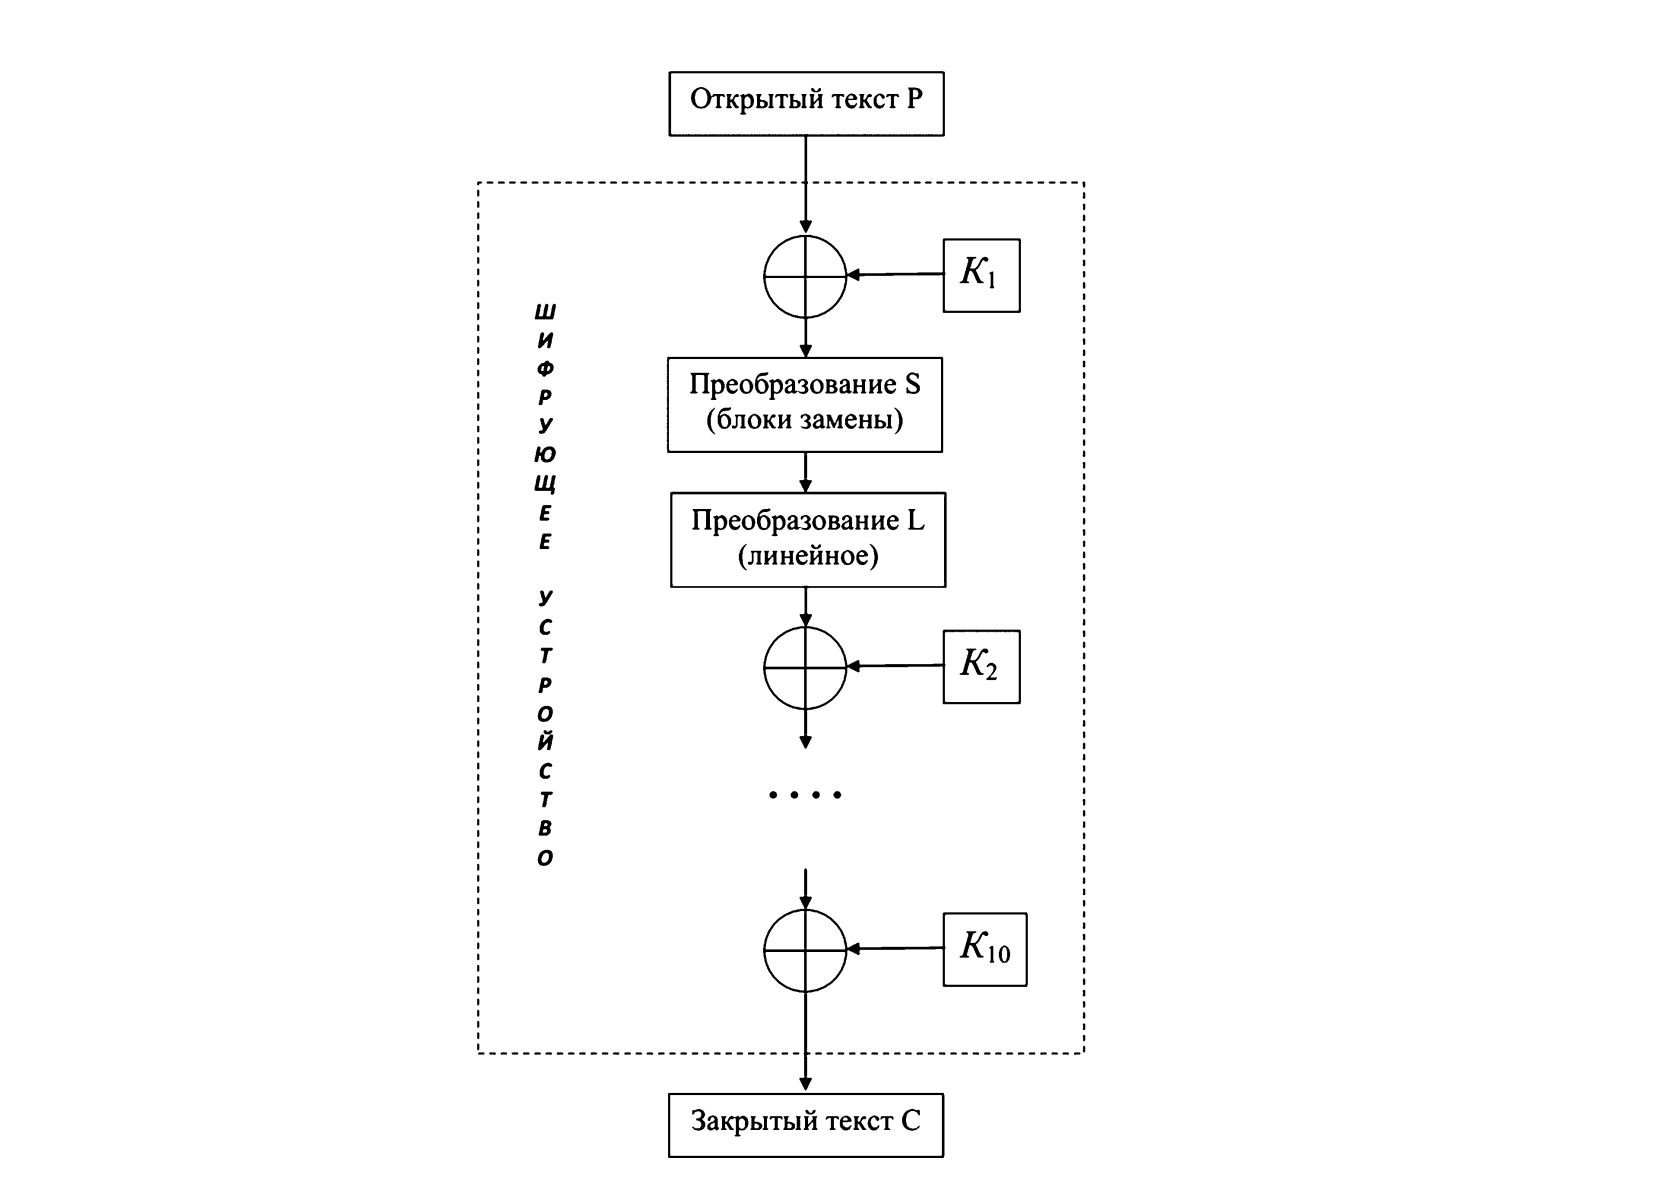
\includegraphics[width=0.99\linewidth]{example/kuznechik1.png} } 

\caption{Схема шифрования}
\end{figure}

\subsection{Технические характеристики}

\textbf{Блоковый Шифр}: "Кузнечик"\ - это блоковый шифр, что означает, что он шифрует данные блоками фиксированного размера.

\textbf{Размер блока открытого текста}: 128 бит.

\textbf{Длина ключа}: 256 бит.

\textbf{Структура}: Основан на SP-сети (substitution-permutation network - сеть подстановок и перестановок). Шифр получает на вход блок и ключ, далее совершает несколько чередуюищхся раундов, которые состоят из стадий подстановки и стадий перестановки. В «Кузнечике» каждый раунд включает в себя линейное и нелинейное преобразование плюс операцию наложения так называемого итерационного ключа. Всего таких раундов девять и один последний неполный раунд, в котором выполняется только наложение последнего (десятого) итерационного ключа.


\textbf{Количество раундов}: Шифр использует 10 раундов шифрования.

\textbf{Сложность}: Высокая криптостойкость благодаря сложной структуре и длинному ключу.

\subsection{Эксплуатационные характеристики}

\textbf{Программная реализация, скорость работы}: Скорость шифрования и дешифрования в "Кузнечике" зависит от реализации и используемого оборудования. Он эффективно работает на современных процессорах, особенно при оптимизации на аппаратном уровне. Скорость может варьироваться, но обычно она достаточно высока для большинства приложений. Например для программной реализации SSE-LS-4 (процессор Core i7-6700) она составляет 360 МБ/с ~\cite{speed}


\textbf{Аппаратная реализация}: в ~\cite{appspeed} предстален анализ глубины аппаратной реализации (определяющим параметром производительности таких реализаций
является глубина схемы, под глубиной понимается длина максимального
простого пути схемы):

Глубина одного раунда Кузнечика не превосходит 24. Общая глубина не превосходит 218. Количество уровней логики на бит 1.7. В сравнении с шифрами Магма, AES-256, DES и 3DES, Кузнечик имеет самую большую глубину одного раунда, однако при этом его показатель количества уровней логики на бит минимален и практически совпадает с AES-256. 

\textbf{Применение}: Широко используется в государственных и военных приложениях в России, также подходит для использования в коммерческих системах для обеспечения высокого уровня защиты данных.
В ~\cite{gost2015} приводится следующее описание, касательно области применения:

Настоящий стандарт определяет алгоритмы базовых блочных шифров, которые применяются
в криптографических методах обработки и защиты информации, в том числе для обеспечения конфиденциальности, аутентичности и целостности информации при ее передаче, обработке и хранении в автоматизированных системах.
Определенные в настоящем стандарте алгоритмы криптографического преобразования предназначены для аппаратной или программной реализации, удовлетворяют современным криптографическим требованиям и по своим возможностям не накладывают ограничений на степень секретности защищаемой информации.
Стандарт рекомендуется использовать при создании, эксплуатации и модернизации систем обработки информации различного назначения.

\textbf{Безопасность}: Предполагается, что шифр обладает высокой устойчивостью к криптоаналитическим атакам, включая дифференциальный и линейный криптоанализ, хотя полная оценка его безопасности требует времени и дополнительных исследований.

\subsection{Атака внесением ошибок на шифр}
Описание атаки основано на статье ~\cite{atack1}

\textbf{Угроза}: сброс в ноль некоторых бит внутреннего состояния некоторого регистра шифрующего устройства путем физического вмешательства.

\textbf{Модель нарушителя}: 
Атакующий имеет доступ к регистрам устройства шифрования: он не знает их значения, но может обнулить состояние конкретного регистра в конкретный момент времени;

Атакующий может неограниченное число раз подавать на вход шифрующему устройству различные открытые тексты и получать соответствующие зашифрованные сообщения;

Устройство шифрования в своей реализации использует известные блоки перестановок, предложенные в стандарте;

Внутри устройства шифрования хранится ключ K, который используется для шифрования, и атакующий стремится узнать значение K.

\textbf{Алгоритм}: Для нахождения i-ого байта ключа $K_1$, можно вносить ошибку в i-ый
байт обрабатываемого блока, после его прохождения через блок преобразования S, перебирая различные входные сообщения до тех пор, пока не получим ошибку, не повлекшую изменений. Ошибка, не повлекшая изменений - та, в результате внесения
которой в процесс шифрования, полученный зашифрованный текст не отличается от исходного.

Если возникает ошибка, не повлекшая изменений, при обнулении некоторого байта обрабатываемого сообщения после его прохождения через S-блоки, значит, соответствующий байт до попадания в S-блок былравен $S^{−1}(0)$.

Следовательно i-ый байт ключа $K_1$ тогда может быть найден по формуле:
$K_1[i] = P[i] \otimes S^{−1}(0)$, 
где $P[i]$ — i-ый байт открытого текста, $S^{−1}(0)$ — обратная перестановка
от нулевого байта (прообраз нуля в блоке замены).
Таким образом, если выполнить данную атаку для каждого из 16-ти
байт итерационного ключа K1, можно полностью узнать его значение.

\textbf{Оценка числа операций, необходимых для реализации атаки}: $2^{13}$ (для нахождения мастер-ключа).

\textbf{Пути нейтрализации атаки}: Данная атака предполагает физический доступ нарушителя к шифрующему устройству, таким образом, акцентируется внимание на важности защиты аппаратных средств шифрования данных от проникновения и внесения изменений.



\subsection{Атака со связанными ключами}
Используют пары открытый/шифрованный текст, полученные на различных ключах, связанных некоторым соотношением.
В общем случае неэффективны, поскольку требуется производить поиск ключей с
заданным соотношением.
Вследствие сложной ключевой развертки атака применима только к варианту шифра с уменьшенным числом раундов и упрощенной ключевой разверткой.

Анализ атаки со связанными ключами на 5 раундов приведен в статье ~\cite{atack2};

Требуемая память – $2^{30}$

Вычислительная сложность – $2^{32}$

\subsection{Алгебраические атаки с мультимножествами}
Анализ атаки на 7 из 9 раундов приведен в статье ~\cite{atack3}

Требуемая память – $2^{140}$

Вычислительная сложность – $2^{155}$

\subsection{Атака "встреча посередине"\ }
Анализ атаки на 6 из 9 раундов приведен в статье ~\cite{atack4}

Требуемая память – $2^{218}$ по 128 бит

Вычислительная сложность – $2^{213}$

\section{Заключение}


В результате анализа блокового шифра ГОСТ 34.12-2018 "Кузнечик"\, можно сформулировать ряд выводов относительно его эксплуатационных аспектов, криптографической устойчивости и практического применения: 

"Кузнечик"\ демонстрирует высокую скорость работы и подходит как для коммерческого использования, так и для государственных нужд.

С точки зрения криптографической стойкости, рассмотренный шифр показывает хорошие результаты против известных методов криптоанализа. 

Таким образом, "Кузнечик"\ представляет собой высокоэффективный и надежный блоковый шифр, сочетающий в себе продвинутую скорость обработки и значительную криптографическую устойчивость. Однако, учитывая динамично развивающийся характер криптографической среды, необходимо обеспечить его непрерывное обновление и адаптацию для поддержания соответствующего уровня защиты данных в долгосрочной перспективе.








\label{sec:minted}
% \show\MINTED
\if \MINTED\empty
% do nothing, minted is off
\else \inputminted{python}{code.py} \fi
\end{document}
%%% Local Variables:
%%% mode: latex
%%% TeX-master: t
%%% End:
